% Results chapter body. Included by thesis.tex under \chapter{RESULTS}.
% This is an \input fragment, not a standalone document.

\section{Economic}
\label{sec:results-economic}

For nine of the twelve participants the APM session cost more in US-dollar-equivalent than the Spec-kit session, as Table~\ref{tab:cost-cohort} reports. The paired cost difference is the APM session cost minus the Spec-kit session cost, and all three summaries of its typical size are positive. The median and the Hodges-Lehmann estimate fall close together, and the mean of the differences is somewhat higher. The Wilcoxon interval does not include zero, so the cohort-level direction holds. Its width, however, leaves the size of the difference imprecise.

\begin{table}[H]
  \centering
  \caption{Paired cost difference across the cohort, APM minus Spec-kit, in US dollars, at 95.8\% coverage.}
  \label{tab:cost-cohort}
  \begin{tabular}{rrrrrr}
    \toprule
    $n$ & Sign ($+$/$-$) & Median & HL & Mean & CI \\
    \midrule
    12 & 9 / 3 & $+6.10$ & $+6.10$ & $+7.14$ & $[+0.42, +14.14]$ \\
    \bottomrule
  \end{tabular}
\end{table}

The mean being higher than the median shows that a few large differences pull the typical size up, rather than the differences being spread evenly, as Figure~\ref{fig:cost-overall} shows. These large values concentrate in one model group, so the cost difference is read next within each model.

\begin{figure}[H]
  \centering
  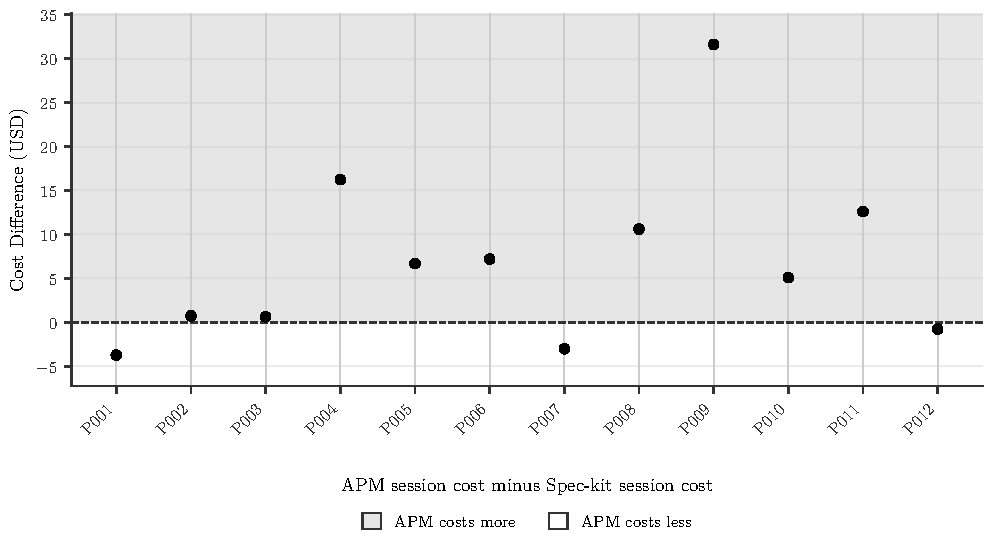
\includegraphics[width=0.85\textwidth]{figures/economic/cost_overall.pdf}
  \caption{Per-participant cost difference, APM minus Spec-kit, in US dollars. A point in the shaded region marks a participant for whom APM cost more.}
  \label{fig:cost-overall}
\end{figure}

The cost difference behaved very differently between the two model groups, set out in Table~\ref{tab:cost-model} and shown in Figure~\ref{fig:cost-by-model}. Among the participants who worked with Opus, five of the six APM sessions cost more, and the difference was large on all three summaries. The median and the Hodges-Lehmann estimate sit close together, with the mean a little above. Among the participants who worked with Sonnet the difference was small on all three summaries and mixed in direction, pointing to the two frameworks costing about the same for that group.

The Opus group also varied widely, from one session where APM cost about four dollars less to one where it cost about thirty-two dollars more. At six participants the confidence interval is wide and includes zero, with its bounds coinciding with those two extremes because at that sample size the interval reaches the smallest and largest differences rather than bounding the estimate more tightly. The Sonnet interval is similarly wide. Opus is the more expensive of the two models, so its differences fall on a larger dollar scale. Those large Opus values pulled the full-cohort summaries up, so the cohort-level cost difference comes mostly from the Opus group.

\begin{table}[H]
  \centering
  \caption{Paired cost differences within each model group, APM minus Spec-kit, in US dollars, at 96.9\% coverage.}
  \label{tab:cost-model}
  \begin{tabular}{lrrrrrr}
    \toprule
    Model & $n$ & Sign ($+$/$-$) & Median & HL & Mean & CI \\
    \midrule
    Opus & 6 & 5 / 1 & $+11.75$ & $+11.89$ & $+12.60$ & $[-3.73, +32.01]$ \\
    Sonnet & 6 & 4 / 2 & $+0.42$ & $+1.25$ & $+1.68$ & $[-2.72, +7.22]$ \\
    \bottomrule
  \end{tabular}
\end{table}

\begin{figure}[H]
  \centering
  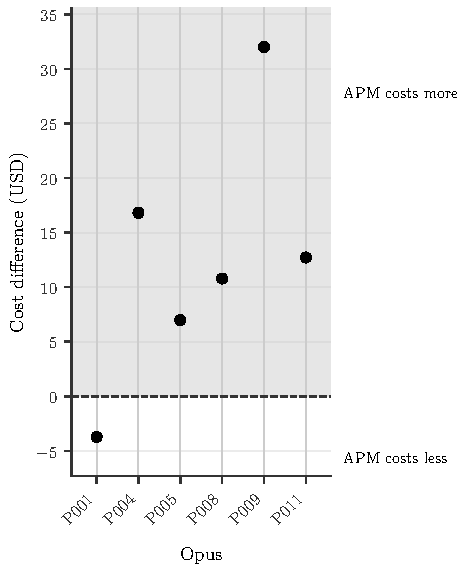
\includegraphics[width=0.49\textwidth]{figures/economic/cost_opus.pdf}\hfill
  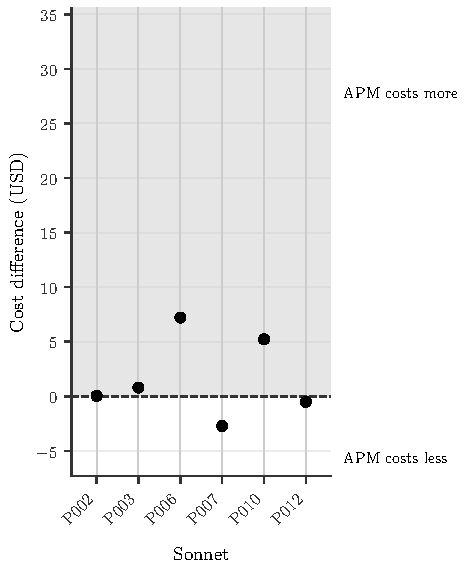
\includegraphics[width=0.49\textwidth]{figures/economic/cost_sonnet.pdf}
  \caption{Per-participant cost difference within each model, APM minus Spec-kit, in US dollars, on a shared scale.}
  \label{fig:cost-by-model}
\end{figure}

The two frameworks divided their spending differently across the task's two phases. As Table~\ref{tab:cost-phase} sets out, APM's planning phase cost less than Spec-kit's and its implementation phase cost more.\footnote{A small residual the parser records as an ``other'' phase, session activity outside either framework's workflow phases, accounts for under one percent of cost and a difference indistinguishable from zero, and is omitted.} Both phase differences exclude zero. The implementation excess was the larger of the two and set the direction of the overall difference. The pattern held in both models, stronger for the Opus group and slighter for the Sonnet group. The per-model split is given in Table~\ref{tab:cost-phase-model} in Appendix~\ref{app:cost-breakdowns}.

\begin{table}[H]
  \centering
  \caption{Paired cost differences by phase, APM minus Spec-kit, in US dollars, at 95.8\% coverage.}
  \label{tab:cost-phase}
  \begin{tabular}{lrrrrrr}
    \toprule
    Phase & $n$ & Sign ($+$/$-$) & Median & HL & Mean & CI \\
    \midrule
    Planning & 12 & 2 / 10 & $-3.77$ & $-4.89$ & $-5.17$ & $[-8.84, -1.44]$ \\
    Implementation & 12 & 10 / 2 & $+9.41$ & $+10.01$ & $+12.21$ & $[+4.10, +22.94]$ \\
    \bottomrule
  \end{tabular}
\end{table}

Within an APM session the cost divided across the three agent roles in the same shape under both models, as Table~\ref{tab:cost-role} details. The Planner and the Manager, the roles that plan the work and coordinate it rather than carry it out, cost on the same order as each other, each a fraction of the Worker's. The bulk of an APM session's cost therefore fell on the agents actually doing the implementation part of the implementation phase. Every role cost more under Opus than under Sonnet, matching the model's higher rate, while the order and rough proportions stayed the same.

\begin{table}[H]
  \centering
  \caption{Cost by agent role within the APM sessions, by model, in US dollars.}
  \label{tab:cost-role}
  \begin{tabular}{llrrr}
    \toprule
    Model & Role & Median & HL & Mean \\
    \midrule
    Opus & Planner & 5.50 & 5.85 & 6.53 \\
    Opus & Manager & 7.35 & 7.31 & 6.97 \\
    Opus & Worker & 21.76 & 21.80 & 22.91 \\
    Sonnet & Planner & 2.67 & 2.67 & 2.66 \\
    Sonnet & Manager & 2.68 & 2.68 & 2.62 \\
    Sonnet & Worker & 9.54 & 9.25 & 9.21 \\
    \bottomrule
  \end{tabular}
\end{table}

The cost difference also divides by token category, the kind of token each dollar paid for, as Table~\ref{tab:cost-token} reports. As Section~\ref{sec:context-windows-and-context-decay} described, each call reprocesses the whole session so far, and caching lowers the price of the tokens that repeat. Under both frameworks Claude Code caches almost all of that prompt, so uncached input was negligible, a few cents either way, and the framework's effect falls on the cache and output categories rather than on fresh input.

The two cache-write rows separate the main agents the user works in from the subagents those agents dispatch. Claude Code writes the one-hour cache for a main agent and the five-minute cache for a subagent. The one-hour writes therefore reflect the framework comparison most directly, since the framework sets how many main agents the user opens.

Two categories drove the difference: output and one-hour writes. APM produced more output than Spec-kit in all but one session and wrote more to the one-hour cache in every session, and for both categories the cohort confidence interval does not include zero. Both differences were larger under Opus than under Sonnet. The cache-read difference was mixed across the cohort, and its confidence interval includes zero. APM read more from the cache than Spec-kit under Opus, and less under Sonnet. The five-minute writes, the subagent cache, were a small positive difference. The per-model split of all five categories is given in Table~\ref{tab:cost-token-model} in Appendix~\ref{app:cost-breakdowns}.

\begin{table}[H]
  \centering
  \caption{Paired cost differences by token category, APM minus Spec-kit, in US dollars, at 95.8\% coverage.}
  \label{tab:cost-token}
  \begin{tabular}{lrrrrrr}
    \toprule
    Category & $n$ & Sign ($+$/$-$) & Median & HL & Mean & CI \\
    \midrule
    Input & 12 & 7 / 5 & $+0.00$ & $+0.00$ & $+0.01$ & $[-0.00, +0.01]$ \\
    Output & 12 & 11 / 1 & $+2.24$ & $+2.20$ & $+2.32$ & $[+1.15, +3.40]$ \\
    Cache read & 12 & 7 / 5 & $+1.16$ & $+1.20$ & $+1.82$ & $[-2.33, +6.03]$ \\
    Cache write (5-minute) & 12 & 10 / 2 & $+0.07$ & $+0.07$ & $+0.05$ & $[-0.00, +0.13]$ \\
    Cache write (1-hour) & 12 & 12 / 0 & $+2.67$ & $+2.50$ & $+2.92$ & $[+1.28, +4.65]$ \\
    \bottomrule
  \end{tabular}
\end{table}

Lastly, session order did not reverse the cost difference. APM cost more than Spec-kit whether participants met it first or second, in four of the six who used it first and five of the six who used it second. Table~\ref{tab:cost-order} in Appendix~\ref{app:cost-breakdowns} gives the difference within each order. The central difference was larger and more consistent when participants met APM second, but at six participants in each order the intervals are wide and the two orders cannot be told apart. The cost difference therefore tracks the framework rather than the order of the sessions, consistent with the learning-effects examination of Section~\ref{sec:disc-learning-effects}, which finds no measurable carry-over between a participant's two sessions.

Two sections in Chapter~\ref{chap:discussions} read these differences further. Section~\ref{sec:disc-sdd} traces the planning-phase difference to how the two frameworks carry out spec-driven planning. Section~\ref{sec:disc-cost-mechanics} takes up the implementation cost, how distributing the work across several agents shapes where the cost falls and why the two model groups diverge.

\section{Process}
\label{sec:results-process}

The process comparison reads how distributing the work across several agents changed the time each task took and the effort it asked of the user. The session's temporal shape is reported first, its interaction shape second.

\subsection{Temporal Shape}
\label{sec:results-process-time}

An APM session lasted a median of about 119 minutes against Spec-kit's 71, as Table~\ref{tab:proc-duration-fw} reports. APM's durations clustered tightly, with its Hodges-Lehmann estimate and mean close to the median, while Spec-kit's mean and Hodges-Lehmann estimate sat above its median, pulled up by a few long sessions. The two phases divided that time differently. APM's time fell mostly in implementation, at a median of about 77 minutes against Spec-kit's 30, while planning was closer and went the other way, with APM at about 36 minutes against Spec-kit's 49.

\begin{table}[H]
  \centering
  \caption{Per-framework session and phase durations, in seconds, across each framework's twelve sessions.}
  \label{tab:proc-duration-fw}
  \begin{tabular}{llrrr}
    \toprule
    Scope & Framework & Median & HL & Mean \\
    \midrule
    Session & APM & $7136.1$ & $7140.5$ & $7267.2$ \\
     & Spec-kit & $4274.6$ & $4684.6$ & $4810.2$ \\
    \midrule
    Planning & APM & $2153.4$ & $2179.3$ & $2298.9$ \\
     & Spec-kit & $2928.3$ & $2888.2$ & $2903.5$ \\
    \midrule
    Implementation & APM & $4641.5$ & $4790.6$ & $4865.1$ \\
     & Spec-kit & $1779.3$ & $1649.6$ & $1879.8$ \\
    \bottomrule
  \end{tabular}
\end{table}

APM was the longer session for every participant, as Table~\ref{tab:proc-time} reports. Paired within each participant, the difference came to a median of about 36 minutes, close to its Hodges-Lehmann estimate, and its confidence interval excludes zero. The session duration divides into the active turn time, when at least one agent was working, and the inter-turn idle between turns, and both were higher under APM in eleven of the twelve pairs.

\begin{table}[H]
  \centering
  \caption{Paired session-time differences across the cohort, APM minus Spec-kit, in seconds, at 95.8\% coverage. The turn time is the active span, and the inter-turn idle is the residual to the session duration.}
  \label{tab:proc-time}
  \begin{tabular}{lrrrrrr}
    \toprule
    Measure & $n$ & Sign ($+$/$-$) & Median & HL & Mean & CI \\
    \midrule
    Session duration & 12 & 12 / 0 & $+2160.7$ & $+2343.6$ & $+2457.0$ & $[+1394.2, +3594.2]$ \\
    Turn time & 12 & 11 / 1 & $+1834.7$ & $+1868.5$ & $+1860.4$ & $[+935.0, +2845.0]$ \\
    Inter-turn idle & 12 & 11 / 1 & $+674.4$ & $+650.1$ & $+596.7$ & $[+93.5, +1201.8]$ \\
    \bottomrule
  \end{tabular}
\end{table}

The session duration difference held under both models and was wider under Opus than Sonnet. Its split into active and idle time held under both as well, with the active-time gap the wider under Opus. Table~\ref{tab:proc-time-model} of Appendix~\ref{app:process-breakdowns} details the per-model split.

The two phases did not share that difference equally, as Table~\ref{tab:proc-phase} sets out. The implementation phase was longer under APM in every pair, with almost all of the extra time spent in active work, and it set the direction of the whole-session difference. The planning difference was a wash, mixed across participants with an interval spanning zero. The one clear planning contrast is in the active time, where Spec-kit's agent worked longer in eight of the twelve pairs, with an interval excluding zero, while the idle time between turns stood even between the frameworks.

\begin{table}[H]
  \centering
  \small
  \setlength{\tabcolsep}{4pt}
  \caption{Paired phase-time differences, APM minus Spec-kit, in seconds, at 95.8\% coverage. Each phase's duration divides into the active turn time and the inter-turn idle.}
  \label{tab:proc-phase}
  \begin{tabular}{llrrrrrr}
    \toprule
    Phase & Measure & $n$ & Sign ($+$/$-$) & Median & HL & Mean & CI \\
    \midrule
    Planning & Duration & 12 & 5 / 7 & $-539.2$ & $-611.9$ & $-604.6$ & $[-1382.7, +200.9]$ \\
     & Turn time & 12 & 4 / 8 & $-606.5$ & $-612.3$ & $-629.9$ & $[-1116.4, -49.1]$ \\
     & Inter-turn idle & 12 & 7 / 5 & $+98.6$ & $+102.3$ & $+25.2$ & $[-290.7, +314.4]$ \\
    \midrule
    Implementation & Duration & 12 & 12 / 0 & $+2549.0$ & $+2605.0$ & $+2985.3$ & $[+1711.9, +4384.1]$ \\
     & Turn time & 12 & 11 / 1 & $+2337.8$ & $+2357.6$ & $+2464.4$ & $[+1452.2, +3655.5]$ \\
     & Inter-turn idle & 12 & 9 / 3 & $+346.5$ & $+367.0$ & $+520.9$ & $[+59.4, +1095.0]$ \\
    \bottomrule
  \end{tabular}
\end{table}

Splitting the two phase differences by model changed neither result. Table~\ref{tab:proc-phase-model} of Appendix~\ref{app:process-breakdowns} presents the per-model view. The implementation phase was longer under APM in all six pairs of each model, with the typical difference somewhat larger under Sonnet. The planning difference remained mixed in sign under both models, with its interval spanning zero.

Session order did not reverse the duration difference. APM was the longer session in all six pairs whether participants met it first or second, as Table~\ref{tab:proc-order} of Appendix~\ref{app:process-breakdowns} reports. The central difference was somewhat larger when participants met APM first, but at six participants in each order the intervals are wide and the two orders cannot be told apart. The duration difference therefore tracks the framework rather than the order of the sessions.

Within the active time APM could have two or more of its agents working at once, which Spec-kit's single conversation cannot. The participants made little use of it. The agents worked one at a time in five of the twelve sessions, and in the seven where they overlapped the concurrent span was a small part of the active time. Table~\ref{tab:proc-concurrency} in Appendix~\ref{app:process-breakdowns} gives the per-session split.

Figure~\ref{fig:proc-temporal} shows each participant's two sessions as paired bars. The filled lower part of each bar is the active time and the open upper part the idle time, so the full height is the session duration. APM's bars stand taller across the cohort, with its active time consistently larger than its Spec-kit pair.

\begin{figure}[H]
  \centering
  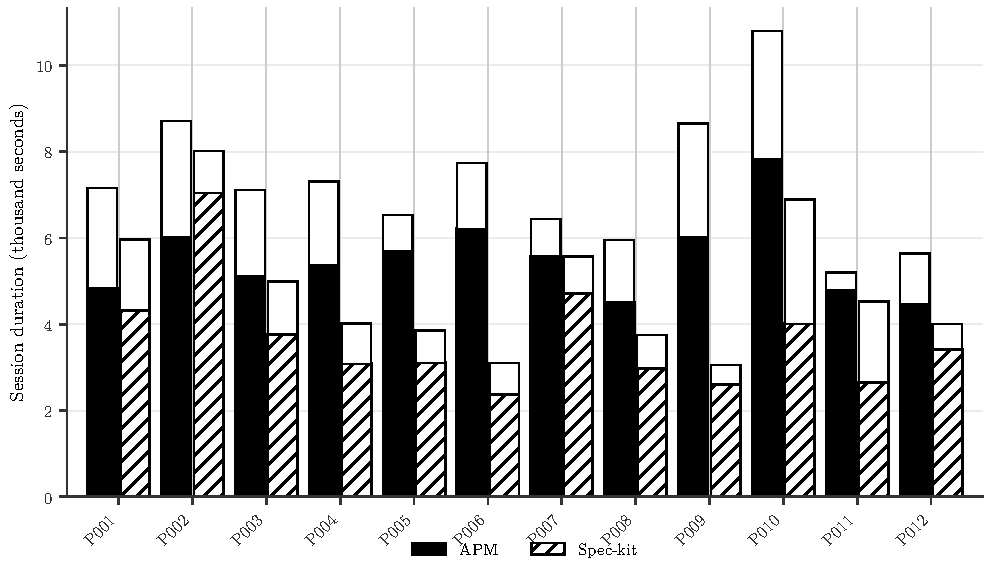
\includegraphics[width=0.85\textwidth]{figures/process/temporal.pdf}
  \caption{Per-participant session temporal shape. Each participant has two bars, APM and Spec-kit; the filled lower segment is the active time, the open upper segment the inter-turn idle, and the full height the session duration.}
  \label{fig:proc-temporal}
\end{figure}

\subsection{Interaction Shape}
\label{sec:results-process-interaction}

\placeholder{Forthcoming. The turn-prompt count compared between frameworks, at the session scope and split by phase, with each framework's typical level reported alongside the paired difference. The per-framework composition of the user's messages across the protocol, short, and standard buckets, by phase, with the mean character length per bucket. The role distribution of the turn prompts across APM's agents. Steering reported as a brief aside. Per-model and per-order breakdowns and the per-participant distributions are deferred to Appendix~\ref{app:process-breakdowns}.}

\section{Functional}
\label{sec:results-functional}

\placeholder{Forthcoming. The total rubric score compared between frameworks by the paired method of the Analysis Plan, the per-section scores decomposing it across the Python and C implementations, and the per-framework score distribution with every session shown. The perceived-effectiveness rating from the questionnaire is reported alongside.}

\section{Perception}
\label{sec:results-perception}

\placeholder{Forthcoming. The eight ordinal rating items compared between frameworks item by item, each by its sign count and median paired difference read with the item's polarity, with the per-framework median profile across the items; the second-session comparative item reported by the framework taken second. Each rating is read against the behaviour it should reflect, descriptively, as the pattern of agreement and divergence.}

\section{Supplementary}
\label{sec:results-supplementary}

\placeholder{Forthcoming. Descriptive per-framework summaries for the supplementary measures: tool success rate, subagent dispatch count, delegated tool-use count, and model-invoked Skill count, per framework and per model, descriptive only and without a paired comparison.}

